\documentclass[a4paper, 11pt]{article}
\usepackage[T1]{fontenc}
\usepackage[utf8]{inputenc}
\usepackage{graphicx}
\usepackage{hyperref}

\hypersetup{
    pdfborder={0 0 0}
}

\newcounter{tc}

\begin{document}

\newcommand{\code}[1]{
    \texttt{#1}
}

\newcommand{\testx}[7]{
	\stepcounter{tc}
	\subsection{Test \thetc: #1} % (fold)
	
	% subsubsection test_1 (end)
	\begin{tabular}{l p{0.7\textwidth}}
    \hline
    \textbf{Test Case Identifier} & \thetc\\
    \hline
    \textbf{Test Item(s)} & \code{#2} $\rightarrow$ \code{#3}\\
    \hline
    \textbf{Input Specification} & #4\\
    \hline
    \textbf{Output Specification} & #5\\
    \hline
    \textbf{Environmental Needs} & #6\\
    \hline
    \textbf{Test Description} & #7\\
    \hline
	\end{tabular}
}

\title{Integration Test Plan Document}

\author{M. Albanese, M. Bianchi, A. Carlucci}

\maketitle
\newpage{}
\tableofcontents{}

\newpage{}

\section{Introduction}
% \subsection{Revision History} 
% \label{sub:revision_history}

\subsection{Purpose} 
\label{sub:purpose}
The purpose of this document, the Integration Test Plan Document (ITPD), is to describe how integration tests are to be performed. The tests that will be described here will mainly focus on the flow of information between different modules rather than on the modules themselves.
In particular, it describes the adopted methodologies, the sets of all tests to be performed, the tools that will be used during the whole process.

\subsection{Scope} % (fold)
\label{sub:scope}
The system will be an optimization of a pre-existing, non-software solution for renting taxis already in use in the city. The new system will let users to rent or reserve a taxi through a mobile or a web application and will also let taxi drivers to take care of the users' requests in a more simple and effective way. In addition to a better user interface, the new system will focus on a smarter organization of the vehicles deployed in each city zone, resulting in a more efficient service for the citizens.

% subsection scope (end)

\subsection{List of definitions and abbreviations} 
\label{sub:list_of_definitions_and_abbreviations}

\begin{description}
    \item[First] The first item
    \item[Second] The first item 
\end{description}

\section{Integration Strategy} 
\label{sec:integration_strategy}

\subsection{Entry Criteria} 
\label{sub:entry_criteria}
Several entry criteria must be met before Integration Testing phase. 
First of all, each component that will be integrated must be - of course - coded. After development phase, each module must successfully pass \textbf{unit testing}, which will guarantee .... TODO ...

\subsection{Elements to be integrated} 
\label{sub:elements_to_be_integrated}

\begin{figure}[htb]
    \centering
    %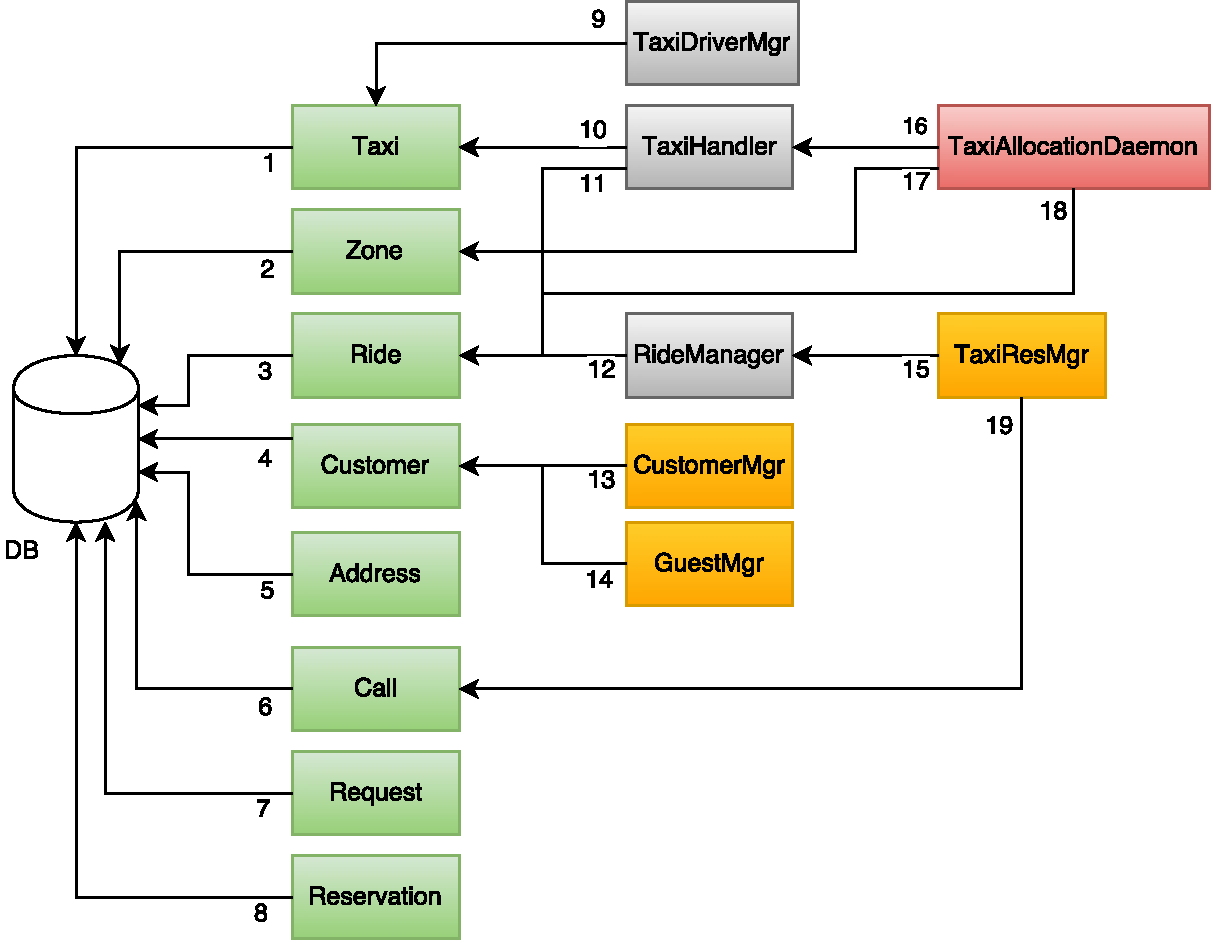
\includegraphics[width=1.2\textwidth]{img/elements.pdf}
    \label{fig:testplan}
\end{figure}


\begin{table}
    \centering
    \begin{tabular}{| l | l | p{0.35\textwidth} | p{0.3\textwidth} |}
    \hline
    \textbf{ID} & \textbf{Component} & \textbf{Subsystem} \\
    \hline
    1 & GuestManager & Client\\
    \hline
    2 & Customer & Client\\
    \hline
    3 & CustomerManager & Client\\
    \hline
    4 & Address & TaxiRes\\
    \hline
    5 & Call & TaxiRes\\
    \hline
    6 & Reservation & TaxiRes\\
    \hline
    7 & Request & TaxiRes\\
    \hline
    8 & Ride & TaxiRes\\
    \hline
    9 & TaxiResManager & TaxiRes\\
    \hline
    10 & RideManager & TaxiRes\\
    \hline
    11 & TaxiAllocationDaemon & TaxiAllocation\\
    \hline
    12 & Zone & TaxiAllocation\\
    \hline
    13 & TaxiHandler & TaxiAllocation\\
    \hline
    14 & Taxi & TaxiDriver\\
    \hline
    15 & TaxiDriverManager & TaxiDriver\\
    \hline
    \end{tabular}
    \caption{List of all components to be integrated}
    \label{tab:components-integration}
\end{table}

\subsection{Integration Testing Strategy} 
\label{sub:integration_testing_strategy}
The strategy that will be adopted is the so-called \textbf{bottom-up} approach. An incremental approach is fundamental, in order to prevent all shortcomings that are typical to Big Bang approach (you have to wait until all modules are complete, localizing the faulty components can be difficult, some interfaces could be missed easily during testing...).
We decided to choose bottom-up over top-down because there are many components at the lower levels (see Figure~\ref{fig:testplan}); this means that only few drivers, if any, are needed.


\subsection{Sequence of Component/Function Integration} 
\label{sub:sequence_of_component_function_integration}

\begin{table}
    \centering
    \begin{tabular}{| l | l | l | l | l |}
    \hline
    \textbf{Test ID} & \textbf{Component 1} & \textbf{Subsystem 1} & \textbf{Component 2} & \textbf{Subsystem 2} \\
    \hline
    1 & Taxi & TaxiDriver & DBMS & DBMS \\
    \hline
    2 & Zone & TaxiAllocation & DBMS & DBMS \\
    \hline
    3 & Ride & TaxiReservation & DBMS & DBMS \\
    \hline
    4 & Customer & Client & DBMS & DBMS \\
    \hline
    5 & Address & TaxiReservation & DBMS & DBMS \\
    \hline
    6 & Call & TaxiReservation & DBMS & DBMS \\
    \hline
    7 & Request & TaxiReservation & DBMS & DBMS \\
    \hline
    8 & Reservation & TaxiReservation & DBMS & DBMS \\
    \hline
    9 & TaxiDriverMgr & TaxiDriver & Taxi & TaxiDriver \\
    \hline
    10 & TaxiHandler & TaxiAllocation & Taxi & TaxiDriver \\
    \hline
    11 & TaxiHandler & TaxiAllocation & Ride & TaxiReservation \\
    \hline
    12 & RideManager & TaxiReservation & Ride & TaxiReservation \\
    \hline
    13 & CustomerManager & Client & Customer & Client \\
    \hline
    14 & GuestManager & Client & Customer & Client \\
    \hline
    15 & TaxiResManager & TaxiReservation & RideManager & TaxiReservation \\
    \hline
    16 & TaxiAllocationDaemon & TaxiAllocation & TaxiHandler & TaxiAllocation \\
    \hline
    17 & TaxiAllocationDaemon & TaxiAllocation & Zone & TaxiAllocation \\
    \hline
    18 & TaxiAllocationDaemon & TaxiAllocation & Ride & TaxiReservation \\
    \hline
    19 & TaxiResManager & TaxiReservation & Call & TaxiReservation \\
    \hline
    \end{tabular}
    \caption{List of all components to be integrated}
    \label{tab:components-integration}
\end{table}

\subsubsection{Software Integration Sequence} 
\label{ssub:software_integration_sequence}

\subsubsection{Subsystem Integration Sequence} 
\label{ssub:subsystem_integration_sequence}

\section{Individual Steps and Test Description} 
\label{sub:individual_steps_and_test_description}

\testx{NAME}{TaxiDriver}{DBMS}{INPUT}{OUTPUT}{ENV. NEEDS}{TEST DESCRIPTION}

\section{Tools and Test Equipment Required} 
\label{sub:tools_and_test_equipment_required}

\section{Program Stubs and Test Data Required} 
\label{sub:program_stubs_and_test_data_required}


\appendix

\clearpage
\addcontentsline{toc}{section}{References}

\begin{thebibliography}{9}
\bibitem{bib:assignment} Prof. Di Nitto.
\emph{????}.
\end{thebibliography}

\vfill

% \section*{Hours spent}
% \begin{figure}[htb]
%     \centering
%     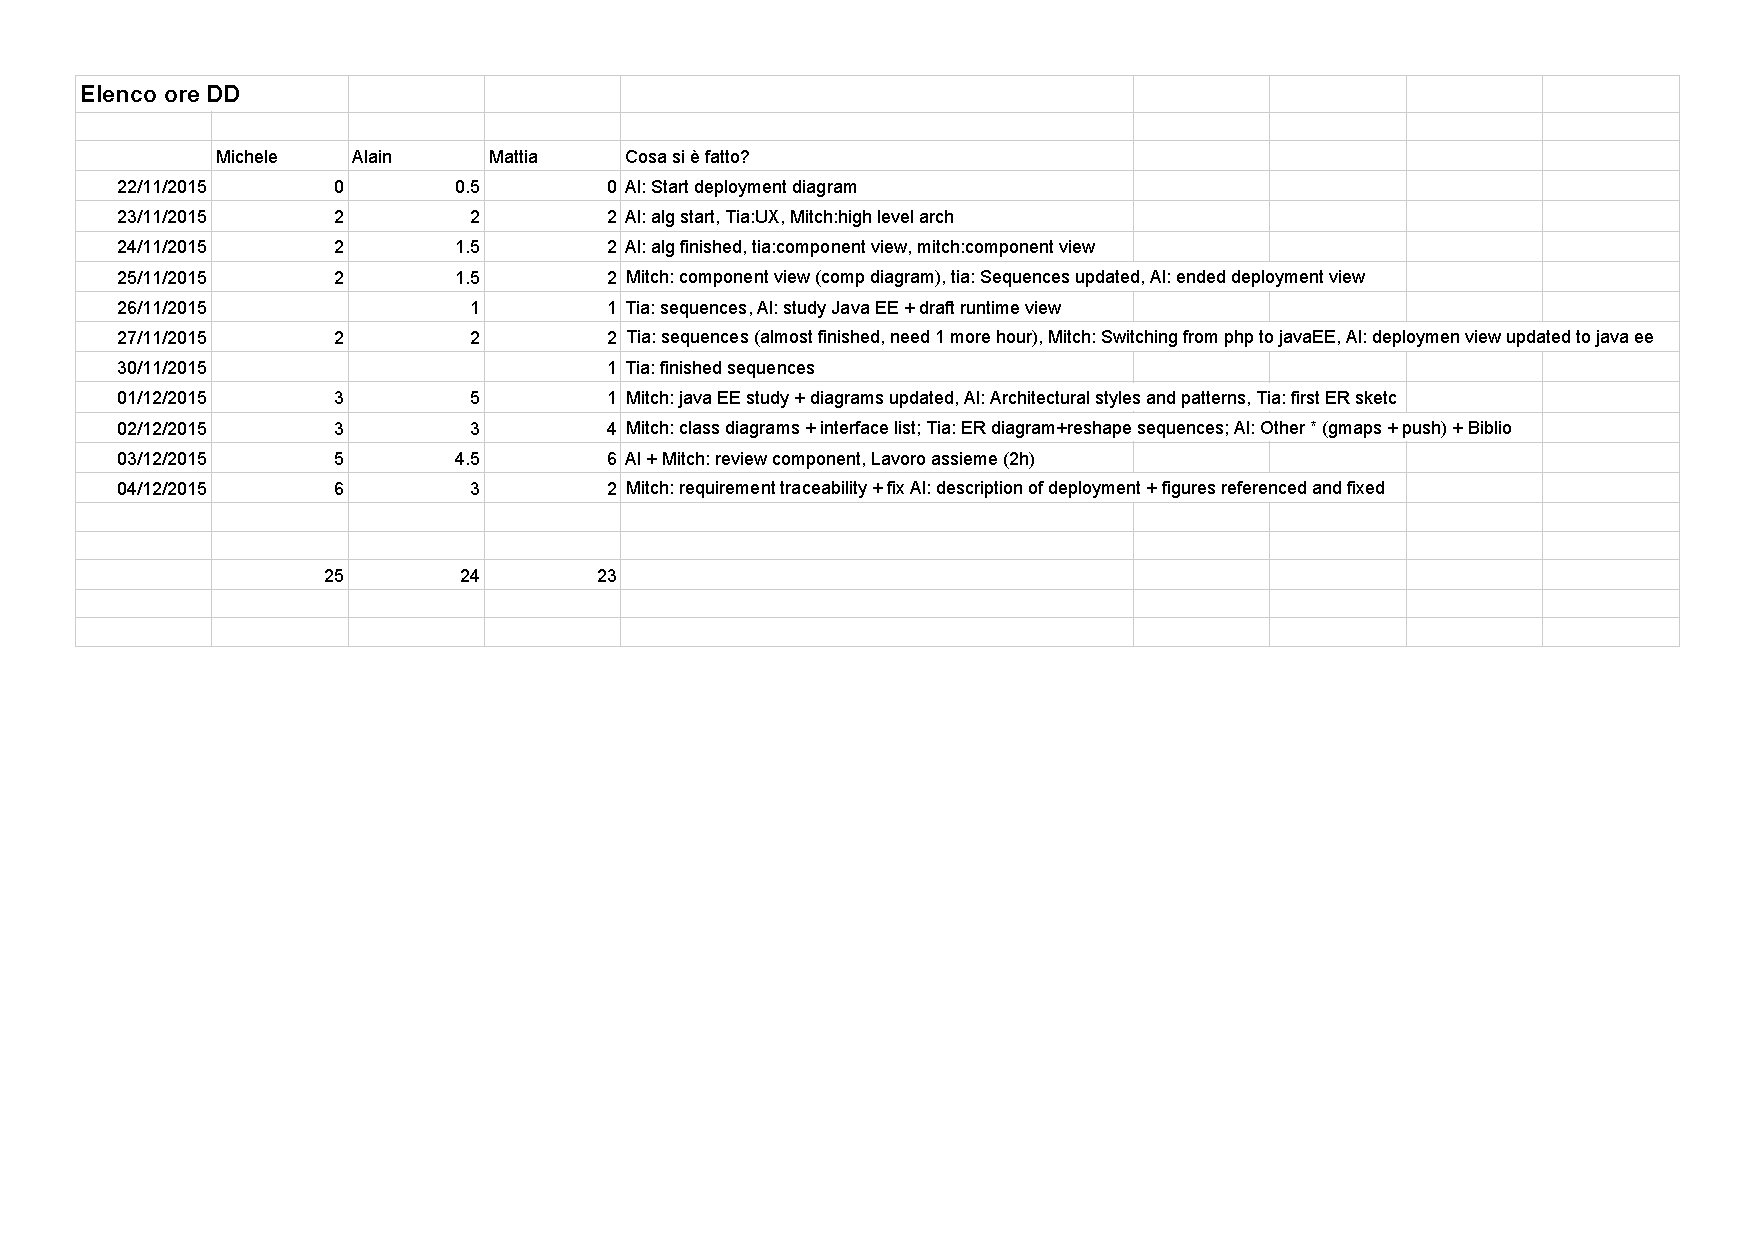
\includegraphics[width=1.2\textwidth]{img/hours.pdf}
%     \label{fig:hours}
% \end{figure}

\end{document}
